%Chapter 2

\renewcommand{\thechapter}{2}

\chapter{Image Texture Analysis}

\section{Texture Analysis Using GLCM Algorithm}

\subsection{Overview}
Grey-Level Co-occurrence Matrix (GLCM) is a common method to represent the distance and angular spatial relationship over the image with a whole segment or sub-segment of specific size. It is created from the array of pixels of an image. Texture is a term to describe an image in another way. The texture measurements of GLCM is firstly proposed by Haralick in the 1970s for image classification\cite{Haralick}. And then, it is widely applied into many fields to solve some specific problems such as the classification of breast lesions on ultrasound (BUS) images\cite{Gomez} and the analysis for synthetic aperture radar (SAR) imagery\cite{Umasankar}. In general, GLCM is a statistic method for calculating the frequency between the pixel of reference and its neighbor. It is created by counting the total number of pairs occurred in the array of pixels. Each pair consists of the reference pixel value and its corresponding neighbor pixel value. Given the symbol $G_{(i,j)}$ which represents the element in GLCM,  we have parameter i that means the reference pixel value and j that means the corresponding neighbor pixel value of the parameter i. In creating a GLCM, there are two major parameters that need to be considered, angle direction and offset. The angle direction of GLCM specifies the possible location of the neighbor pixel regard to its reference pixel. General speaking, there are four basic GLCM directions that are the $0^0$ degree $P_0$, the $90^0$ degree $P_{90}$ and the diagonal degree that includes the $45^0$ representing bottom left to to top right $P_{45}$ and the $135^0$ representing top left to bottom right $P_{135}$ shown in Figure 2.1. 
\begin{figure}[!t]
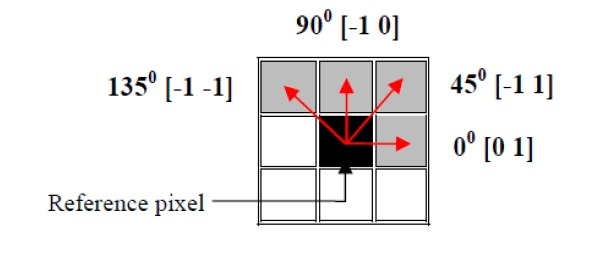
\includegraphics{GLCM_direction_sample}
\caption{GLCM angle directions for calculating textural features\cite{Biswajit}}
\end{figure}
In addition, by considering the symmetric property, the value of each element is doubled. In general, there is the fifth GLCM created by considering the average over created GLCM along with four angle directions. Offset means the distance between reference pixel value and its neighbor. Given $E_{(i,j)}$ which is the element in the array of pixels representing an image, if we consider $E_{(i,j)}$ as reference, the $E_{(i,j+n)}$ where n means the value of the offset is the neighbor in horizontal direction from left to right. Similarly, the the $E_{(i-n,j+n)}$ is the neighbor in diagonal direction from bottom left to top right, the $E_{(i-n,j)}$ is the neighbor in vertical direction from bottom to top, and the $E_{(i-n,j-n)}$ is the neighbor from bottom right to top left.\par
For example, given a 3-by-6 array  
\begin{align*}
I = 
\begin{bmatrix}
& 1 & 1 & 5 & 6 & 8 & 8 &\\
& 2 & 3 & 5 & 7 & 0 & 2 &\\
& 0 & 2 & 3 & 5 & 6 & 7 &
\end{bmatrix}
\end{align*}
it represents a sub-region of an image with pictorial information. GLCM is a m-by-m matrix where m is the gray levels of an image. For image I, since the pixel value ranges from 0 to 8, the gray level of image I is 9. Thus, a 9-by-9 matrix is created as a part of the whole GLCM in $0^0$ angle direction with offset 1. Under this circumstance, considering $E_{(1, 1)} = 1$ as the reference pixel value, its neighbor is $E_{(1, 2)} = 1$. Thus, the $G_{(1,1)}$ is currently equal to 1. In the meantime, we can find that the $G_{(0, 2)} = 2$, because when we treat the pixel value 0 as the reference, the pixel value 2 as the corresponding neighbor appears twice, which are $E_(2,6)$ and $E_(3,2)$.    
\begin{table}[!h]
\begin{center}
\renewcommand{\arraystretch}{0.5}
\begin{tabular}{c | c c c c c c c c c|}
 \backslashbox{\textit{reference}}{\textit{neighbor}} & 0 & 1 & 2 & 3 & 4 & 5 & 6 & 7 & 8 \\
\hline
 0 & 0 & 0 & 2 & 0 & 0 & 0 & 0 & 0 & 0 \\
 1 & 0 & 1 & 0 & 0 & 0 & 0 & 0 & 0 & 0 \\
 2 & 0 & 0 & 0 & 2 & 0 & 0 & 0 & 0 & 0 \\
 3 & 0 & 0 & 0 & 0 & 0 & 2 & 0 & 0 & 0 \\
 4 & 0 & 0 & 0 & 0 & 0 & 0 & 0 & 0 & 0 \\
 5 & 0 & 0 & 0 & 0 & 0 & 0 & 2 & 1 & 0 \\
 6 & 0 & 0 & 0 & 0 & 0 & 0 & 0 & 1 & 1 \\
 7 & 1 & 0 & 0 & 0 & 0 & 0 & 0 & 0 & 0 \\
 8 & 0 & 0 & 0 & 0 & 0 & 0 & 0 & 0 & 1 \\
\end{tabular}
\caption{The sub-region of GLCM in 0 degree (offset = 1)}
\end{center}
\end{table}
By counting all reference pixel values, we achieve the GLCM shown in Table 2.1. Similarly, we create the different GLCM in the rest three directions shown in Table 2.2, Table 2.3 and Table 2.4.
\begin{table}[!h]
\begin{center}
\renewcommand{\arraystretch}{0.5}
\begin{tabular}{c | c c c c c c c c c|}
 \backslashbox{\textit{reference}}{\textit{neighbor}} & 0 & 1 & 2 & 3 & 4 & 5 & 6 & 7 & 8 \\
\hline
 0 & 0 & 0 & 0 & 1 & 0 & 0 & 0 & 0 & 1 \\
 1 & 0 & 0 & 0 & 0 & 0 & 0 & 0 & 0 & 0 \\
 2 & 0 & 1 & 0 & 0 & 0 & 1 & 0 & 0 & 0 \\
 3 & 0 & 0 & 0 & 0 & 0 & 1 & 0 & 1 & 0 \\
 4 & 0 & 0 & 0 & 0 & 0 & 0 & 0 & 0 & 0 \\
 5 & 1 & 0 & 0 & 0 & 0 & 0 & 1 & 0 & 0 \\
 6 & 0 & 0 & 1 & 0 & 0 & 0 & 0 & 0 & 0 \\
 7 & 0 & 0 & 0 & 0 & 0 & 0 & 0 & 0 & 1 \\
 8 & 0 & 0 & 0 & 0 & 0 & 0 & 0 & 0 & 0 \\
\end{tabular}
\caption{The sub-region of GLCM in 45 degree (offset = 1)}
\end{center}
\begin{center}
\renewcommand{\arraystretch}{0.5}
\begin{tabular}{c | c c c c c c c c c|}
 \backslashbox{\textit{reference}}{\textit{neighbor}} & 0 & 1 & 2 & 3 & 4 & 5 & 6 & 7 & 8 \\
\hline
 0 & 0 & 0 & 1 & 0 & 0 & 0 & 0 & 0 & 1 \\
 1 & 0 & 0 & 0 & 0 & 0 & 0 & 0 & 0 & 0 \\
 2 & 0 & 1 & 0 & 1 & 0 & 0 & 0 & 0 & 1 \\
 3 & 0 & 1 & 0 & 0 & 0 & 1 & 0 & 0 & 0 \\
 4 & 0 & 0 & 0 & 0 & 0 & 0 & 0 & 0 & 0 \\
 5 & 0 & 0 & 0 & 0 & 0 & 1 & 0 & 1 & 0 \\
 6 & 1 & 0 & 0 & 0 & 0 & 0 & 0 & 0 & 0 \\
 7 & 0 & 0 & 1 & 0 & 0 & 0 & 1 & 0 & 0 \\
 8 & 0 & 0 & 0 & 0 & 0 & 0 & 0 & 0 & 0 \\
\end{tabular}
\caption{The sub-region of GLCM in 90 degree (offset = 1)}
\end{center}
\end{table}
\begin{table}
\begin{center}
\renewcommand{\arraystretch}{0.5}
\begin{tabular}{c | c c c c c c c c c|}
  \backslashbox{\textit{reference}}{\textit{neighbor}} & 0 & 1 & 2 & 3 & 4 & 5 & 6 & 7 & 8 \\
\hline
 0 & 0 & 0 & 0 & 0 & 0 & 0 & 1 & 0 & 0 \\
 1 & 0 & 0 & 0 & 0 & 0 & 0 & 0 & 0 & 0 \\
 2 & 0 & 0 & 1 & 0 & 0 & 0 & 0 & 0 & 1 \\
 3 & 0 & 1 & 0 & 1 & 0 & 0 & 0 & 0 & 0 \\
 4 & 0 & 0 & 0 & 0 & 0 & 0 & 0 & 0 & 0 \\
 5 & 0 & 1 & 0 & 0 & 0 & 1 & 0 & 0 & 0 \\
 6 & 0 & 0 & 0 & 0 & 0 & 0 & 0 & 1 & 0 \\
 7 & 1 & 0 & 0 & 0 & 0 & 1 & 0 & 0 & 0 \\
 8 & 0 & 0 & 0 & 0 & 0 & 0 & 0 & 0 & 0 \\
\end{tabular}
\caption{The sub-region of GLCM in 135 degree (offset = 1)}
\end{center}
\end{table}
For all tables from 2.1 to 2.4, the 
Finally, through adding these four GLCM together and dividing it by 4, we have the fifth GLCM.

\subsection{Texture Measurements of GLCM}
The texture measures of GLCM are calculated from the normalized GLCM. To achieve the normalized GLCM, each value in GLCM is divided by the total number of occurrences in the GLCM. Normally, the total number of occurrences is the amount of valid reference pixel. For instance, if we create the GLCM from the image I along with the $0^0$ direction with offset 1, the total number of occurrences is 15 because the reference pixels in the last column have no neighbors. Some basic functions will be used in calculating the texture features of GLCM\cite{Haralick}. Assuming that the parameter G represents the number of gray levels, the basic functions are defined as follow:\\
The probability of i as the reference pixel value in a gray-scale image:
\begin{equation}
    p_x(i) = \sum_{j=0}^{G-1}p(i,j) 
\end{equation}
The probability of j as the neighbor pixel value in a gray-scale image:
\begin{equation}
    p_y(j) = \sum_{i=0}^{G-1}p(i,j)
\end{equation}
The probability of k which is the summary of reference and neighbor pixel value:
\begin{equation}
    p_{x+y}(k) = \sum_{i=0}^{G-1}\sum_{j=0}^{G-1} p(i,j) \; where\; k = i + j\;(k=0,1,\ldots,2G-2)
\end{equation}
The probability of k which is the difference of reference and neighbor pixel value:
\begin{equation}
    p_{x-y}(k) = \sum_{i=0}^{G-1}\sum_{j=0}^{G-1} p(i,j) \; where\; k = |i - j|\;(k=0,1,\ldots,G-1)
\end{equation}
The mean value of $p_x$:
\begin{equation}
\mu_x = \sum_{i=0}^{G-1}ip_x(i)=\sum_{i=0}^{G-1}\sum_{j=0}^{G-1} ip(i,j)
\end{equation}
The standard deviation of $p_x$:
\begin{equation}
\sigma_x = \sqrt{\sum_{i=0}^{G-1}(i-\mu_x)^2p_x(i)}
\end{equation}
The mean value of $p_y$:
\begin{equation}
\mu_y = \sum_{j=0}^{G-1}jp_j(j)=\sum_{i=0}^{G-1}\sum_{j=0}^{G-1} jp(i,j)
\end{equation}
The standard deviation of $p_y$:
\begin{equation}
\sigma_y = \sqrt{\sum_{j=0}^{G-1}(j-\mu_y)^2p_y(j)}
\end{equation}
Consequently, due to the normalized GLCM and the basic functions listed above, the texture feature parameters of GLCM are defined as follow\cite{Haralick}:\\
1. Energy, Homogeneity, Angular Second Moment(ASM): 
\begin{equation}
ASM = \sum_{i=0}^{G-1}\sum_{j=0}^{G-1}\{p(i,j)\}^2
\end{equation}
The feature ASM is used to measure the homogeneity of an image\cite{Peng}. The value of ASM is usually more than $G^{-2}$ but less than 1. If a GLCM only has a few but relatively high value of $p(i,j)$, the homogeneous scene contains only a few gray levels\cite{Albregtsen}.\\
2. Inertia, Contrast(CON):
\begin{equation}
CON = \sum_{k=0}^{G-1}k^2p_{x-y}(k)
\end{equation}
The feature CON is used to measure the local difference within an image. Its value depends the position of pixel. In general, the more elements away from the diagonal, the higher value the feature has. Otherwise, the more elements in the diagonal, the lower value it has.\\ 
3. Correlation(COR):
\begin{equation}
COR = \frac{\sum_{i=0}^{G-1}\sum_{j=0}^{G-1}(i-\mu_x)(j-\mu_y)p(i,j)}{\sigma_x\sigma_y} = \frac{\sum_{i=0}^{G-1}\sum_{j=0}^{G-1}(ij)p(i,j)-\mu_x\mu_y}{\sigma_x\sigma_y}
\end{equation}
The feature COR is used to measure the linear dependence of gray levels between the specific position of pixels relative to each other. It depends how an image is organized. The value of COR is more than -1 but less than 1.\\
4. Sum of squares, variance(VAR):
\begin{equation}
VAR = \sum_{i=0}^{G-1}\sum_{j=0}^{G-1}(i-\mu_x)^2p(i,j) \\
    = \sum_{i=0}^{G-1}(i-\mu_x)^2p_x(i)
\end{equation}
The feature VAR measures the degree how the elements differ from the average value of $p(i,j)$. \\
5. Local Homogeneity, Inverse Difference Moment(IDM):
\begin{equation}
IDM = \sum_{i=0}^{G-1}\sum_{j=0}^{G-1}\frac{1}{1+(i-j^2)}p(i,j)
\end{equation}
The feature IDM is affected by the homogeneity of an image, because of the weighting factor $1+(i - j)^2$. Thus, the value is high if the image is homogeneous, while the value is low if the image is inhomogeneous.\\
6. Sum Average(SAV):
\begin{equation}
SAV = \sum_{k=0}^{2G-2}kp_{x+y}(k)
\end{equation}
7. Sum Entropy(SEN):
\begin{equation}
SEN = -\sum_{k=0}^{2G-2}p_{x+y}(k)\log(p_{x+y}(k))
\end{equation}
8. Sum Variance(SVA):
\begin{equation}
SVA = \sum_{k=0}^{2G-2}(k-SEN)^2p_{x+y}(k)
\end{equation}
9. Entropy(ENT)
\begin{equation}
ENT = - \sum_{i=0}^{G-1}\sum_{j=0}^{G-1}p(i,j)\log(p(i,j))
\end{equation}
10. Difference Entropy(DEN):
\begin{equation}
DEN = -\sum_{k=0}^{G-1}p_{x-y}(k)\log(p_{x-y}(k))
\end{equation}
11. Difference Variance(DVA):
\begin{equation}
DVA = \sum_{k=0}^{G-1}k^2p_{x-y}(k)
\end{equation}
12. Dissimilarity(DIS):
\begin{equation}
DIS = \sum_{i=0}^{G-1}\sum_{j=0}^{G-1}|i-j|p(i,j)
\end{equation}
13. Cluster shade(CLS):
\begin{equation}
CLS = \sum_{i=0}^{G-1}\sum_{j=0}^{G-1}(i+j-\mu_x-\mu_y)^3p(i,j) = \sum_{i=0}^{G-1}\sum_{j=0}^{G-1}(i+j-2\mu_x)^3p(i,j)
\end{equation}
14. Cluster prominence(CLP):
\begin{equation}
CLP=\sum_{i=0}^{G-1}\sum_{j=0}^{G-1}(i+j-\mu_x-\mu_y)^4p(i,j) = \sum_{i=0}^{G-1}\sum_{j=0}^{G-1}(i+j-2\mu_x)^4p(i,j)
\end{equation}
15. Minimum probability(MIP):
\begin{equation}
MIP = \min(p(i,j))
\end{equation}
16. Maximum probability(MAP):
\begin{equation}
MAP=max(p(i,j))
\end{equation}
17. Mean(MEA):
\begin{equation}
MEA = \sum_{i=0}^{G-1}i\sum_{j=0}^{G-1}p(i,j) = \mu_x
\end{equation}
18. relative minimum pixel intensity(IMIN):
\begin{equation}
IMIN = \frac{min(J(x,y))}{mean(J(x,y))}
\end{equation}
19. relative maximum pixel intensity(IMAX):
\begin{equation}
IMAX = \frac{max(J(x,y))}{mean(J(x,y))}
\end{equation}
20. Mean value of pixel intensity(IMEA):
\begin{equation}
IMEA = mean(J(x,y))
\end{equation}
where J(x,y) represents the 12-bit diffraction image before normalization. Based on Haralick's research\cite{Thati}, the texture features defined above are categorized into three groups named as \textit{Contrast}, \textit{Uniformity} or \textit{Orderliness} of pixels, and \textit{Correlation} and \textit{statistic} over the pixels. In Group 1, the measures of Contrast includes CON, DIS, IDM, VAR, SVA and DVA. In Group 2, the measures of Uniformity or Orderliness of pixels consist of MAP, ASM, ENT, DEN, SEN, CLS and CLP. In group 3, the measures of Correlation and other descriptive statistics contain COR, MIP, MEA, IMIN, IMAX, IMEA and SAV.\par
These feature parameters facilitate representing an image from the textural level. For example, given two different types of diffraction images taking both from camera with s-polarizer in front of as the Figure 2.2 shown, we examine three basic feature parameters from different group. The feature CON in group 1 describes the difference moment of image pixel matrix by measuring the amount of local variations present in an image. As for the images shown in Figure 2.2, the CON value of Cell image is 2.511395, while the value of Debris image is 104.8141, which is calculated using equation 2.10. The Debris image has larger CON value than the Cell image because the Cell image has less amount of local variations than the Debris image as the Figure 2.2 shown. The feature ASM in group 2 describes the degree of homogeneity that an image has by measuring the total number of dominant gray-tone transitions. Through calculation, the value of Cell image is 0.031834, whereas the value of Debris image is 0.000838. Due to the fact that the Cell image has very fewer dominant gray-tone transitions than the Debris image, the ASM of Cell image is higher than the Debris image. Another feature COR in group 3 describes the gray-tone linear-dependencies by considering the amount of linear structure across the image. The Debris image has lower value than the Cell image because the Debris image contains noise sample which is usually uncorrelated. In the meanwhile, by comparing the COR value of the Debris image along different directions, the values along $0^0$ and $90^0$ are higher than the values along $45^0$ and $135^0$ because the Debris image has a certain amount of linear structure along these two lines across it. 
\begin{figure}[!t]
\centering
  \begin{subfigure}[b]{0.4\textwidth}
    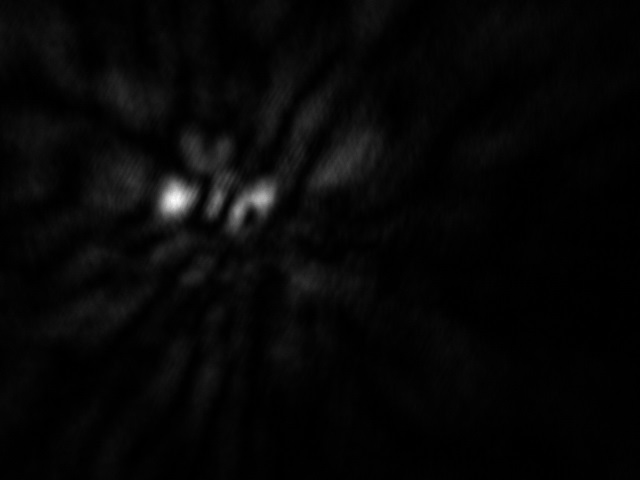
\includegraphics[width=\textwidth]{diffraction_image/2015040117594700116-2}
    \caption{Cell image}
  \end{subfigure}
  \begin{subfigure}[b]{0.4\textwidth}
    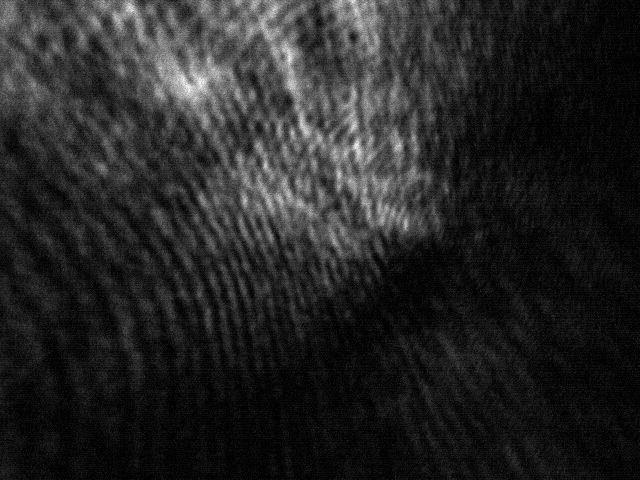
\includegraphics[width=\textwidth]{diffraction_image/2015040117594700009-2}
    \caption{Debris image}
  \end{subfigure}
  \caption{Two diffraction images with different types captured with s-polarizer}
\end{figure}
\section{Development of GLCM Feature Calculation Application}
\subsection{Problem Statement}
Since the GLCM as a texture analysis approach is so popular, some tools provide the built-in method to create GLCM, such as MATLAB. However, for users who do not have the experience on MATLAB, it is hard for them to utilize the built-in method there. Even though users have little knowledge or experience of MATLAB, it is inconvenient to implement a script for extracting GLCM texture feature parameters. Thus, a developed application is necessary to be implemented. From the requirement perspective, the application shall allow users to specify the image folder so that the application can automatically process all images in that folder. The application also shall allow users to customize the offset value and the direction for creating the GLCM. To expand the function, the application should enable users to have the choices that the application presents feature parameters in single direction or combination of directions or the feature parameters normalized by all processed directions. Finally, the application shall automatically combine an image pair as a feature parameter example.  
\subsection{Class Diagram and GLCM Application Implementation}
\begin{figure}[!h]
\begin{center}
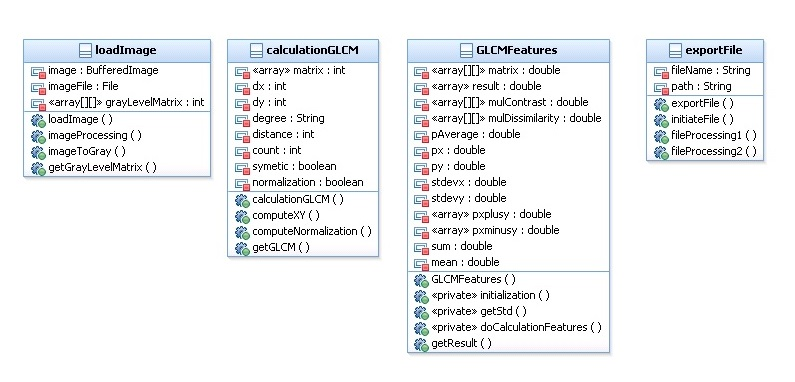
\includegraphics[width=4.25in]{class_diagram}
\end{center}
\renewcommand{\baselinestretch}{1}
\small\normalsize
\begin{quote}
\caption{The major classes for GLCM feature calculation application}
\label{fig2.2}
\end{quote}
\end{figure}
\renewcommand{\baselinestretch}{2}
\small\normalsize
Based on the problem statement above, the application should comprise several components which are loading images, converting into 2D matrix, computing GLCM based on the 2D matrix, calculating features from GLCM, and exporting comma-separated values (CSV) file that is used to store the desirable result. Therefore, the major classes shown in Figure 2.3 are constructed to represent the attributes and operations within the application. To process the massive amount of images, the application loops the procedure consisting of class loadImage, class calculationGLCM, and class GLCMFeatures until no image remained. During each loop, all calculated features are stored using ArrayList method. Finally, class exportFile extracts all features from ArrayList and conducts them into CSV file.\par
In this application, class loadImage is implemented by applying the Application Program Interface (API) Image I/O in JAVA library. The API provides a way loading the image into its BufferedImage formats. It supports with built-in methods for GIF, PNG, JPEG, BMP, and WBMP which are some different format of image data. In JAVA, the BufferedImage which is a subclass of Image class describes an image with an accessible buffer of image data. Within the BufferedImage class, it is constructed by the raster of image data that represents a rectangle array of pixels. Thus, through applying these APIs, the image data is processed and generate a rectangle array of pixels whose size is due to the resolution of the image. for example, if the resolution of an image is 640x480, the raster of the image data is a 640-by-480 array of pixels. In the meantime, the range of image pixel depends on its color depth. For instance, the highest pixel of an 8-bit image data is 256. \par
The calculationGLCM class takes the array of pixels that is the output of loadImage class as input and create the specific GLCM due to other input parameters such as distance and angular. The mechanism for this class is going through all elements in the array of pixels, and for each element, finding its corresponding neighbor element with specific conditions. Meanwhile, if an element has no neighbor, it contributes nothing to GLCM. As a result, given an m-by-n array of pixels
\begin{align*}
I = 
\begin{bmatrix}
E(0,0) & E(0,1) & \ldots & E(0,n-1) \\
\vdots &         &         & \vdots \\
E(d,0) & E(d,1) & \ldots & E(d,n-1) \\
\vdots &         &         & \vdots \\
E(m-1,0) & E(m-1,1) & \ldots & E(m-1,n-1) 
\end{bmatrix}
\end{align*} where d is the offset value and considering the exception problem in programming,
to calculate GLCM along 0 degree direction, a two dimension loop that counting the frequency starts from the element $E(0,0)$ and ends at the element $E(m-1, n-d)$; to calculate GLCM along 45 degree direction, the loop starts from the element $E(d,0)$ and ends at the element $E(m-1, n-d)$; to calculate GLCM along 90 degree direction, the loop starts from the element $E(d,0)$ and ends at the element $E(m-1, n-1)$; to calculate GLCM along 135 degree direction, the loop starts from the element $E(d,d)$ and ends at the element $E(m-1, n-1)$. 
By applying class GLCMFeatures, all texture features are calculated from the GLCM created through class calculationGLCM. In this class, the method initialization() is implemented to calculate parameters $p_x(i)$, $p_y(j)$, $p_{x+y}(k)$, $p_{x-y}(k)$, $\mu_x$, $\mu_y$, $\sigma_x$ and $\sigma_y$ due the equations from 2.1 to 2.8. Then, we implement the doCalculationFeatures() method that is responsible for calculating the 17 texture features of an image which are listed from equation 2.9 to 2.25.\par
Finally, the class exportFile is implemented for creating the result report in CSV format. General speaking, the common strategy is building a string with the comma. In this case, we utilize the StringBuilder method to construct the string in that format and apply the printWriter function to add it to a specific CSV file. 

\subsection{GLCM Application Verification}
Software verification as a part of software testing is an important procedure to ensure that the software is implemented all requirements. The two primary goals for software testing is finding bugs or defects and getting confidence in the software\cite{Jiantao}. Traditionally, the testing methods are divided into white-box testing that examines the internal structure or workings of a program and black-box testing that examines the functionality without knowing the internal implementation and seeing the source code. To do the black-box testing, test oracle which is a mechanism in software testing to determine whether a test has passed or not\cite{Kaner} is required. in the meanwhile, the test case which includes a set of test data as inputs, the expected outputs, and the execution condition is the central factor that is involved in the use of an oracle. As for the GLCM application, the input is an image and the output is the corresponding texture features based on the image's GLCM for system testing which is a high-level software testing process.
In this thesis research, there are MATLAB scripts implemented for research in selecting features to analyze the diffraction image\cite{Thati} and the C++ tool implemented for calculating texture features from GLCM. To verify them, we consider the black-box testing because tester lacks enough knowledge in MATLAB and C++ programming language. However, by using four diffraction images shown in Figure 2.4 as inputs for the testing process, the calculated texture features are different between these two tools. 
\begin{figure}[!b]
  \begin{subfigure}[b]{0.5\textwidth}
    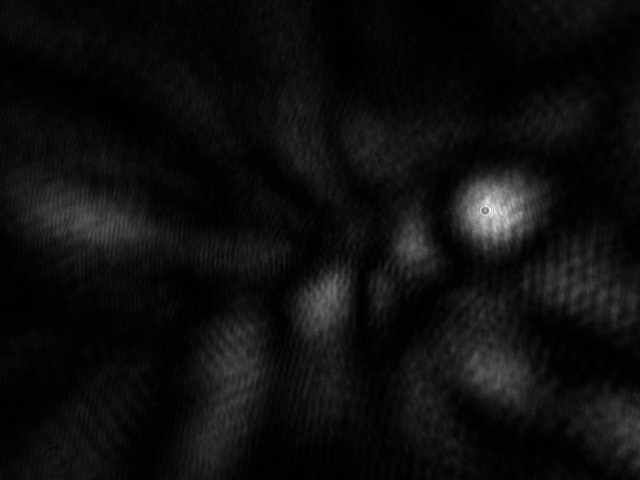
\includegraphics[width=\textwidth]{PicA1000}
    \caption{}
  \end{subfigure}
  \begin{subfigure}[b]{0.5\textwidth}
    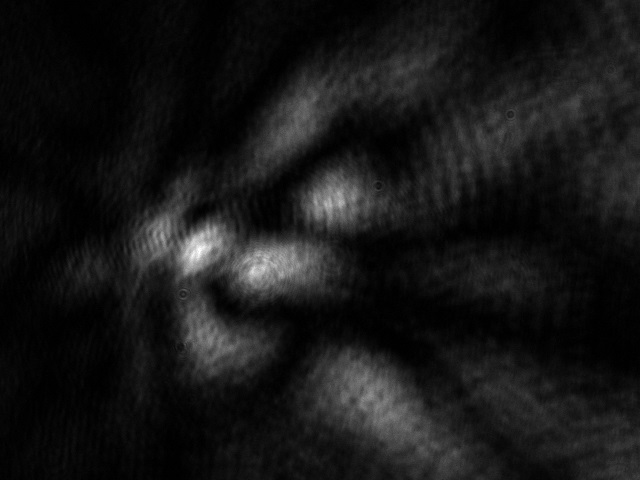
\includegraphics[width=\textwidth]{PicA1001}
    \caption{}
  \end{subfigure}
  \begin{subfigure}[b]{0.5\textwidth}
    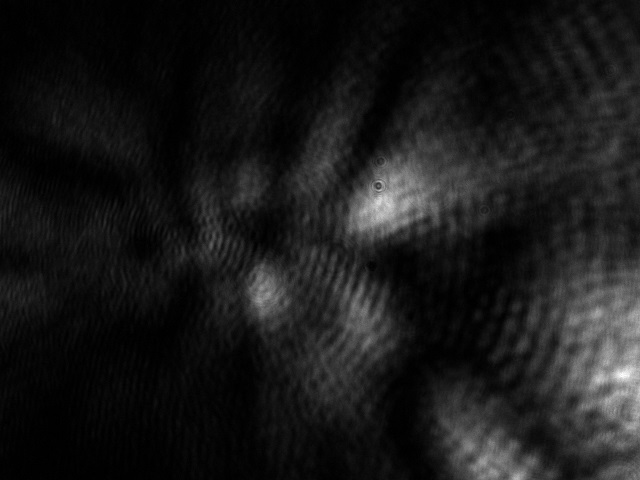
\includegraphics[width=\textwidth]{PicA1002}
    \caption{}
  \end{subfigure}
  \begin{subfigure}[b]{0.5\textwidth}
    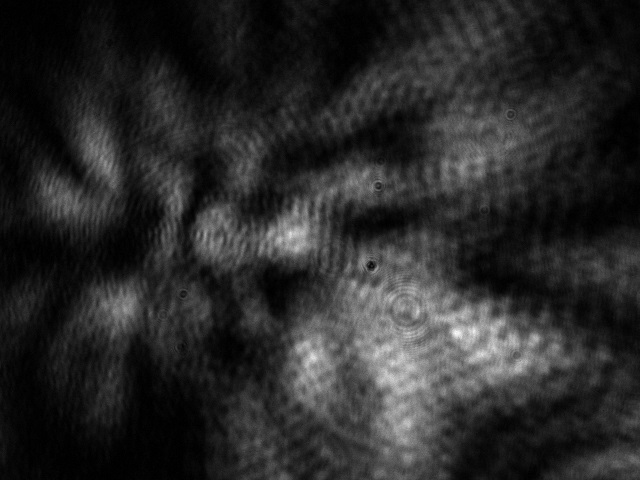
\includegraphics[width=\textwidth]{PicA1003}
    \caption{}
  \end{subfigure}
  \caption{The test input for verifying GLCM applications}
\end{figure}
In Table 2.5, we select five textural features from total 17 features to compare. Based on the comparison of results between MATLAB and C++, we can assume that either one of the code has or both of them have bugs or defects inside so that the requirements are not satisfied well. To prove, another application is implemented in JAVA, which is discussed in previous section, to verify the assumption proposed above. 
\begin{table}[!b]
\begin{center}
\begin{tabular}{||c c c ||}
& Image (a) & \\
\hline
Feature & MATLAB & C++ \\[0.7ex]
\hline\hline
COR & 0.985299 & 0.984588 \\
DIS & 2.20703 & 2.234017 \\
CON & 10.06387 & 10.63786 \\
IDM & 0.380147 & 0.407319 \\
ASM & 0.005497 & 0.013697 \\
\hline
\end{tabular}
\vspace{0.5cm}
\begin{tabular}{||c c c ||}
& Image (b) & \\
\hline
Feature & MATLAB & C++ \\[0.7ex]
\hline\hline
COR & 0.990801 & 0.990473 \\
DIS & 2.459202 & 2.487369 \\
CON & 12.97538 & 13.50661 \\
IDM & 0.364664 & 0.387451 \\
ASM & 0.003817 & 0.009142 \\
\hline
\end{tabular}
\begin{tabular}{||c c c ||}
& Image (c) & \\
\hline
Feature & MATLAB & C++ \\[0.7ex]
\hline\hline
COR & 0.991887 & 0.991633 \\
DIS & 2.626308 & 2.651188 \\
CON & 14.99225 & 15.53600 \\
IDM & 0.355747 & 0.380085 \\
ASM & 0.003739 & 0.009151 \\
\hline
\end{tabular}
\begin{tabular}{||c c c ||}
& Image (d) & \\
\hline
Feature & MATLAB & C++ \\[0.7ex]
\hline\hline
COR & 0.989492 & 0.989358 \\
DIS & 3.956470 & 3.969021 \\
CON & 30.91669 & 31.39502 \\
IDM & 0.254904 & 0.272799 \\
ASM & 0.001061 & 0.002534 \\
\hline
\end{tabular}
\caption {The feature values calculated from MATLAB and C++ for images in Figure 2.4}
\end{center}
\end{table}
At the beginning, the JAVA code is only implemented for calculating the COR, DIS, CON, IDM and ASM texture feature parameters for verification purpose. By using the same four diffraction images shown in Figure 2.4 as test inputs, we unfortunately got another version of result that is different from both MATLAB and C++. In Table 2.6, we present the comparison of result for Figure 2.4(a). 
\begin{table}[!t]
\begin{center}
\begin{tabular}{||c c c c||}
\hline
Feature & MATLAB & C++ & JAVA\\[0.7ex]
\hline\hline
COR & 0.985299 & 0.984588 & 0.962522 \\
DIS & 2.20703 & 2.234017 & 6.818101\\
CON & 10.06387 & 10.63786 & 82.14295 \\
IDM & 0.380147 & 0.407319 & 0.217207 \\
ASM & 0.005497 & 0.013697 & 0.005483\\
\hline
\end{tabular}
\caption{The texture feature results of Figure 2.4(a)}
\end{center}
\end{table}
From this result, we can't prove the assumption until we verify that the JAVA application is implemented to meet requirements. We apply the JUnit testing for major components comprising loadImage, calculationGLCM and GLCMFeatures. Consequently, we construct an 10-by-10 array of pixels ranging from 0 to 9 
\begin{align*}
I = 
\renewcommand{\arraystretch}{0.5}
\begin{bmatrix}
    1 & 6 & 2 & 3 & 9 & 3 & 0 & 6 & 2 & 8\\
    6 & 5 & 4 & 4 & 8 & 6 & 5 & 3 & 3 & 8\\
    0 & 9 & 7 & 0 & 0 & 6 & 8 & 2 & 6 & 7\\
    1 & 6 & 7 & 9 & 7 & 5 & 6 & 4 & 2 & 2\\
    5 & 7 & 1 & 2 & 2 & 6 & 2 & 4 & 7 & 5\\
    1 & 4 & 4 & 1 & 4 & 6 & 3 & 1 & 9 & 0\\
    7 & 4 & 5 & 3 & 5 & 2 & 4 & 5 & 7 & 4\\
    7 & 7 & 4 & 2 & 8 & 1 & 9 & 2 & 3 & 3\\
    7 & 1 & 6 & 4 & 4 & 9 & 1 & 3 & 5 & 1\\
    1 & 1 & 6 & 3 & 9 & 2 & 8 & 5 & 1 & 2
\end{bmatrix}
\end{align*}
as a test input to represent an image. By manually creating GLCM along 0 degree direction from the array of pixels, we achieve the GLCM
\begin{align*}
G_0 = 
\renewcommand{\arraystretch}{0.5}
\begin{bmatrix}
    1&     0&     0&     0&     0&     0&      2&     0&     0&     1\\
    0&     1&     2&     1&     2&     0&     4&     0&     0&     2\\
    0&     0&     2&     2&     2&     0&     2&     0&     3  &   0\\
    1&     1&     0&     2&     0&     2&     0&     0&     1 &    2\\
    0&     1&     2&     0&     3&     2&     1&     1 &    1  &   1\\
    0 &    2  &   1  &   2   &  1  &   0  &   1 &    2&     0  &   0\\
    0&     0&     3&     2&     2&     2&     0&     2&     1  &   0\\
    1&     2&     0&     0&     3&     2&     0&     1 &    0  &   1\\
    0 &    1  &   1   &  0   &  0  &   1 &    1&     0&     0  &   0\\
    1&     1&     2&     1&     0&     0&     0&     2&     0  &   0
\end{bmatrix}
\end{align*}
Based on the GLCM, we calculate the values of texture feature parameters COR, DIS, CON, IDM and ASM which are the expected outputs. Therefore, we create a test case including the test input I and expected output G for the JAVA application that is treated as execution condition. Through the verification process, we achieve the result shown in Table 2.7. 
\begin{table}[!h]
\begin{center}
\begin{tabular}{|| c | c  c | c ||}
\hline
Texture Feature & expected Result & Actual Result & Passed \\
\hline\hline
COR & 0.999965 & 0.999965 & Y \\
DIS & 290.0 & 290.0 & Y \\
CON & 1432.0 & 1432.0 & Y \\
IDM & 22.749199 & 22.749199 & Y\\
ASM & 174.0 & 174.0 & Y\\
\hline
\end{tabular}
\end{center}
\caption{Testing result for JAVA application}
\end{table}
As the table shown, all actual results are matched with expected results, which indicates the JAVA application can satisfy the requirements and achieve the correct feature values. To cover all possible GLCM created along all directions, we perform the same process for 45 degree, 90 degree and 135 degree angle and manually create the GLCM for the rest single direction:
\begin{align*}
G_{45} = 
\renewcommand{\arraystretch}{0.5}
\begin{bmatrix}
     0&     0&     0&     0&     0 &    1&     1&     0&     1&     0\\
     0&     2&     2&     0&     2 &    0&     1&     2&     0&     2\\
     0&     1&     0&     2&     1 &    2&     0&     3&     0&     0\\
     0&     0&     1&     1&     4 &    0&     0&     0&     1&     0\\
     0&     3&     2&     2&     1 &    0&     2&     0&     1&     1\\
     0&     1&     1&     1&     0 &    1&     3&     0&     1&     1\\
     1&     0&     3&     0&     1 &    1&     2&     1&     1&     0\\
     2&     0&     1&     0&     3 &    1&     1&     2&     0&     0\\
     0&     0&     1&     3&     0 &    0&     0&     0&     0&     0\\
     1&     0&     0&     0&     1 &    2&     0&     0&     0&     2
\end{bmatrix}
G_{90} = 
\begin{bmatrix}
     0&     0&     0&     0&     1&     1&     1&     0&     1&     0\\
     1&     1&     2&     1&     1&     2&     0&     3&     0&     1\\
     0&     1&     0&     2&     0&     1&     3&     2&     0&     2\\
     0&     1&     3&     0&     2&     0&     1&     1&     0&     0\\
     1&     1&     4&     2&     2&     1&     0&     1&     1&     0\\
     1&     2&     1&     2&     2&     0&     2&     0&     0&     0\\
     0&     1&     0&     2&     1&     1&     3&     0&     1&     1\\
     1&     1&     1&     0&     2&     0&     1&     3&     1&     1\\
     0&     1&     0&     0&     0&     2&     0&     0&     1&     1\\
     1&     1&     0&     0&     2&     1&     0&     1&     0&     0
\end{bmatrix}
\end{align*}
\begin{align*}
G_{135} = 
\renewcommand{\arraystretch}{0.5}
\begin{bmatrix}
     0&     0&     0&     0 &    2 &    0 &    0 &    1  &   0  &   0\\
     0&     2&     1&     2 &    0 &    1 &    1 &    2  &   0  &   0\\
     0&     0&     1&     0 &    3 &    4 &    1 &    1  &   0  &   1\\
     1&     0&     0&     0 &    1 &    1 &    3 &    1  &   0  &   1\\
     0&     1&     3&     0 &    2 &    1 &    3 &    1  &   1  &   1\\
     1&     3&     2&     2 &    1 &    0 &    0 &    0  &   0  &   0\\
     1&     1&     1&     1 &    0 &    0 &    1 &    2  &   1  &   1\\
     1&     2&     0&     1 &    1 &    1 &    0 &    1  &   0  &   1\\
     0&     0&     1&     2 &    0 &    0 &    1 &    0  &   0  &   1\\
     0&     0&     1&     0 &    2 &    0 &    1 &    1  &   1  &   0
\end{bmatrix}
\end{align*}
Based on these GLCM, we further create the average GLCM from all directions via dividing the sum for each element in GLCM by 4. The average GLCM is 
\begin{align*}
G_{ave} = 
\renewcommand{\arraystretch}{0.5}
\begin{bmatrix}
0.25 &0 &0 &0 &0.75 &0.5 &1 &0.25 &0.5 &0.25\\
0.25 &1.5 &1.75 &1 &1.25 &0.75 &1.5 &1.75 &0 &1.25\\
0 &0.5 &0.75 &1.5 &1.5 &1.75 &1.5 &1.5 &0.75 &0.75\\
0.5 &0.5 &1 &0.75 &1.75 &0.75 &1 &0.5 &0.5 &0.75\\
0.25 &1.5 &2.75 &1 &2 &1 &1.5 &0.75 &1 &0.75\\
0.5 &2 &1.25 &1.75 &1 &0.25 &1.5 &0.5 &0.25 &0.25\\
0.5 &0.5 &1.75 &1.25 &1 &1 &1.5 &1.25 &1 &0.5\\
1.25 &1.25 &0.5 &0.25 &2.25 &1 &0.5 &1.75 &0.25 &0.75\\
0 &0.5 &0.75 &1.25 &0 &0.75 &0.5 &0 &0.25 &0.5\\
0.75 &0.5 &0.75 &0.25 &1.25 &0.75 &0.25 &1 &0.25 &0.5
\end{bmatrix}
\end{align*}
Through operating the calculationGLCM method, all GLCM generated from JAVA application are the same as the expected results. 
Although we confirm that the texture features can be correctly calculated from GLCM, as well as that the GLCM can be created from the array of pixels, it is required to verify whether the array of pixels can represent the image correctly or not. Because of the complexity of image data, it is impossible to manually create the expected output for an image. Instead, we consider using a verified method to generate the expect output from image such as the imread() method in MATLAB. However, by comparing some elements with the same position in the matrix, the values are different. We pick 27-pixel values of image ranging from 10 to 255 in the matrix generated from the imread() method and choose the same number of the pixel value in the same position of a matrix created from JAVA application. Through building a map between each pixel value from MATLAB and its corresponding value from JAVA, we can obviously see the nonlinear line trend shown in Figure 2.5, 
\begin{figure}[!h]
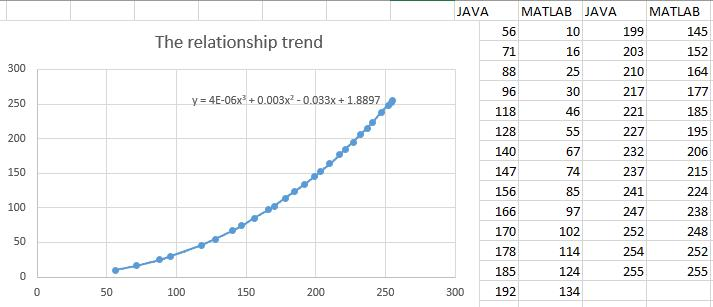
\includegraphics[width = \linewidth]{rgb_statistical}
\caption{The nonlinear relationship between JAVA and MATLAB result}
\end{figure}
which means we fail to create the correct pixel matrix from the image using JAVA application. Through some research, the misuse of the class Color is the reason of getting the wrong matrix. Instead of class Color, class Raster is the correct choice for a Gray-level image. The problem is caused by default color space sRGB, a proposed standard RGB color space, in Color class. Also, in BufferedImage class, the method getRGB() return an integer pixel in default color model TYPE\_INT\_ARGB, while the color model of our images is TYPE\_BYTE\_GRAY. Thus, we replace the Color class with the Raster class. After fixing the defects existing in loadingImage class, we use the Figure 2.4(a) as input to run JAVA application again and receive the new result shown in Table 2.8. 
\begin{table}[!t]
\begin{center}
\begin{tabular}{||c c c c||}
\hline
Feature & MATLAB & C++ & JAVA\\[0.7ex]
\hline\hline
COR & 0.985299 & 0.984588 & 0.985184 \\
DIS & 2.20703 & 2.234017 & 2.2324890\\
CON & 10.06387 & 10.63786 & 10.13244 \\
IDM & 0.380147 & 0.407319 & 0.375932 \\
ASM & 0.005497 & 0.013697 & 0.005439\\
\hline
\end{tabular}
\caption{The texture feature results of Figure 2.4(a) after modification}
\end{center}
\end{table}
From the result, we can see there are still three different version of feature result, but for JAVA application, all components have passed the verification process, and the all possible directions for creating GLCM are covered within the testing procedure. Thus, we can confirm the assumption that both C++ application and MATLAB script contain defects, and the JAVA application can be applied in the future research.

\section{Diffraction Images Pre-Classification and Feature Calculation}
In this experiment, we are provided 6000 diffraction images within which there are 3000 diffraction image pairs. Each image pair contains two diffraction images captured at the same time by two cameras with s-polarizer or p-polarizer placed separately in front of them. All diffraction images we use in the experiment are 8-bit color, so the gray levels of an image are 256 ranging from 0 to 255. In addition, the resolution of these images is 640x480. Thus, the array of pixels is a 640-by-480 matrix with that the maximum number of each element is 255. To identify, the diffraction image pair has the same name as the symbol (-) and different part (1 or 2) after the symbol. For instance, the 2015040718412300745-1.bmp means the p-polarized, whereas the 2015040718412300745-2.bmp means the s-polarized. There is some research using the similar approach to acquiring diffraction images, such as the classification of Jurkat T and Ramos B cells\cite{Feng} and the analysis of cellular objects through diffraction images\cite{Zhang}. \par
The primary goal of this research is to select a model to solve automated classification problem for these diffraction image data. In general, the common strategy is to train computer by using supervised learning algorithm in machine learning. By applying this approach, the computer can attain the ability that classifying massive amount of diffraction image data itself. However, for training process, we have to have the training data set labeled. Therefore, all 3000 diffraction image pairs are pre-classified visually into to three types, Cell, Debris, and Strip. Some image pairs for each group are shown in Figure 2.6, 2.7 and 2.8. 
\begin{figure}[!h]
\centering
  \begin{subfigure}[b]{0.2\textwidth}
    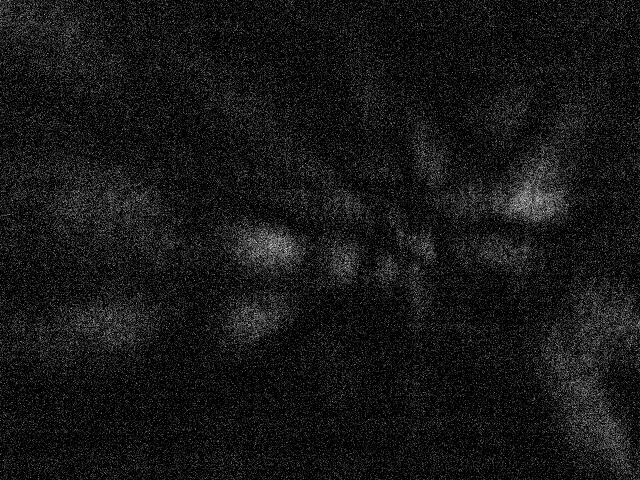
\includegraphics[width=\textwidth]{diffraction_image/2015040117594700171-1}
    \caption{p-polarizer}
  \end{subfigure}
  \begin{subfigure}[b]{0.2\textwidth}
    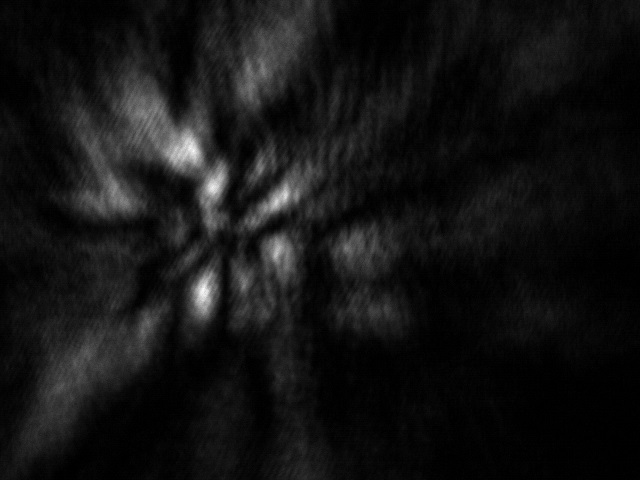
\includegraphics[width=\textwidth]{diffraction_image/2015040117594700171-2}
    \caption{s-polarizor}
  \end{subfigure}
  \begin{subfigure}[b]{0.2\textwidth}
    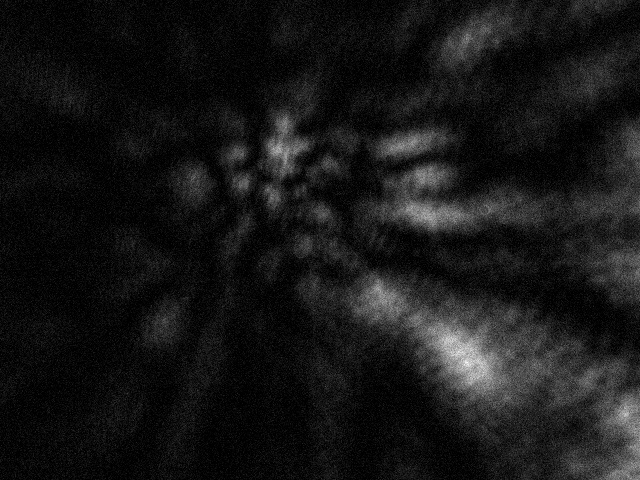
\includegraphics[width=\textwidth]{diffraction_image/2015040117594700185-1}
    \caption{p-polarizer}
  \end{subfigure}
  \begin{subfigure}[b]{0.2\textwidth}
    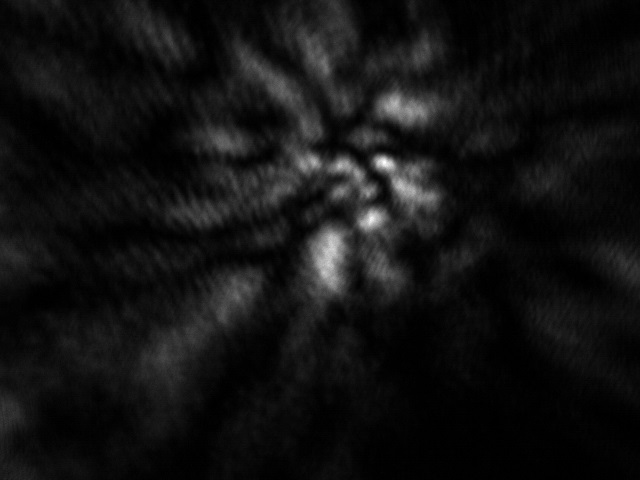
\includegraphics[width=\textwidth]{diffraction_image/2015040117594700185-2}
    \caption{s-polarizor}
  \end{subfigure}
  \caption{Diffraction images classified as Cell type}
\end{figure}
\begin{figure}[!h]
\centering
  \begin{subfigure}[b]{0.2\textwidth}
    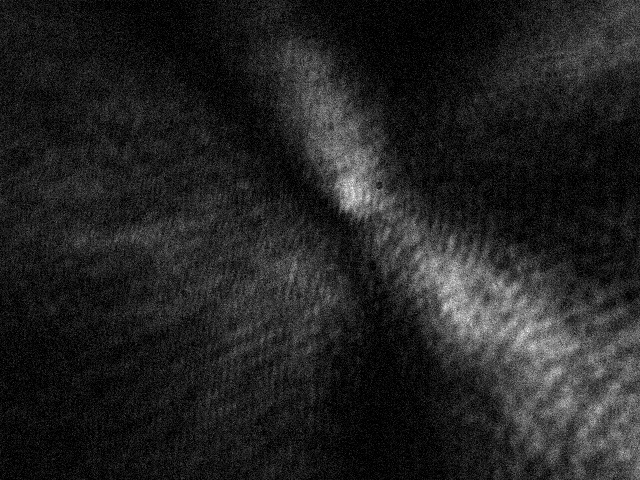
\includegraphics[width=\textwidth]{diffraction_image/2015040117594700004-1}
    \caption{p-polarizer}
  \end{subfigure}
  \begin{subfigure}[b]{0.2\textwidth}
    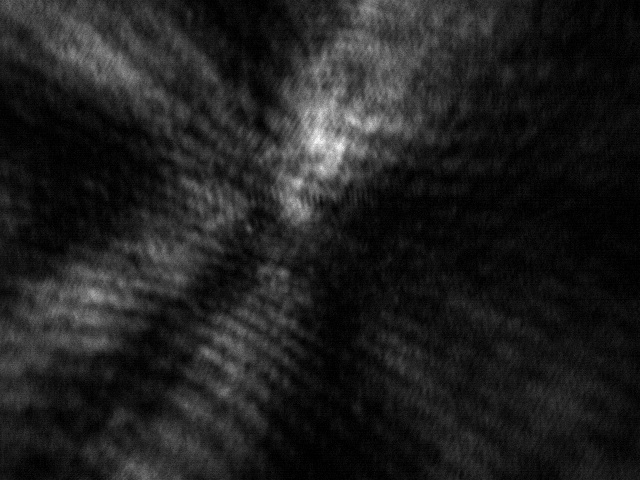
\includegraphics[width=\textwidth]{diffraction_image/2015040117594700004-2}
    \caption{s-polarizor}
  \end{subfigure}
  \begin{subfigure}[b]{0.2\textwidth}
    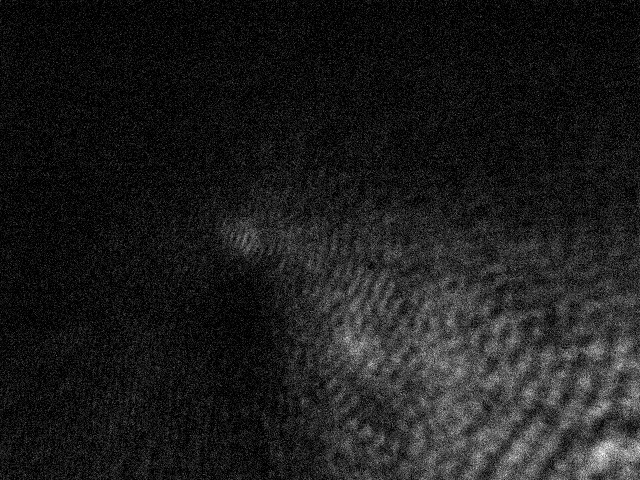
\includegraphics[width=\textwidth]{diffraction_image/2015040117594700050-1}
    \caption{p-polarizer}
  \end{subfigure}
  \begin{subfigure}[b]{0.2\textwidth}
    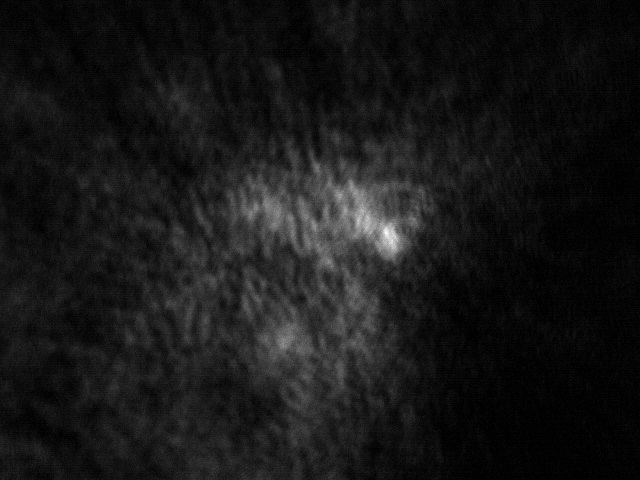
\includegraphics[width=\textwidth]{diffraction_image/2015040117594700050-2}
    \caption{s-polarizor}
  \end{subfigure}
  \caption{Diffraction images classified as Debris type}
\end{figure}
\begin{figure}[!h]
\centering
  \begin{subfigure}[b]{0.2\textwidth}
    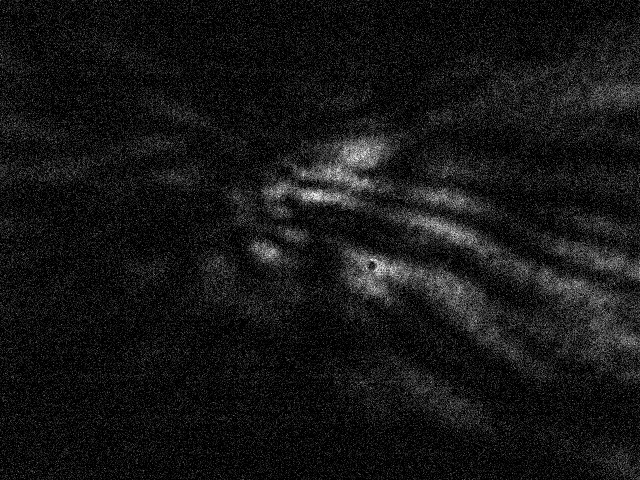
\includegraphics[width=\textwidth]{diffraction_image/2015040117594700071-1}
    \caption{p-polarizer}
  \end{subfigure}
  \begin{subfigure}[b]{0.2\textwidth}
    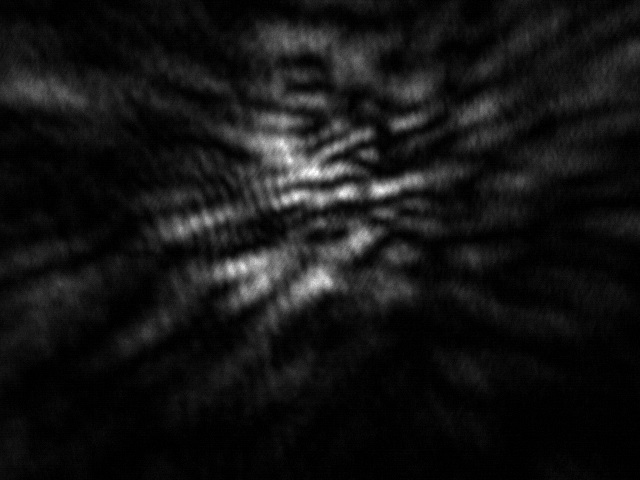
\includegraphics[width=\textwidth]{diffraction_image/2015040117594700071-2}
    \caption{s-polarizor}
  \end{subfigure}
  \begin{subfigure}[b]{0.2\textwidth}
    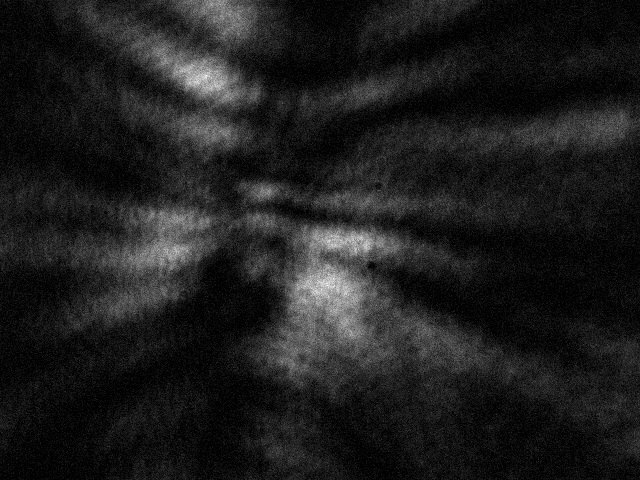
\includegraphics[width=\textwidth]{diffraction_image/2015040117594700158-1}
    \caption{p-polarizer}
  \end{subfigure}
  \begin{subfigure}[b]{0.2\textwidth}
    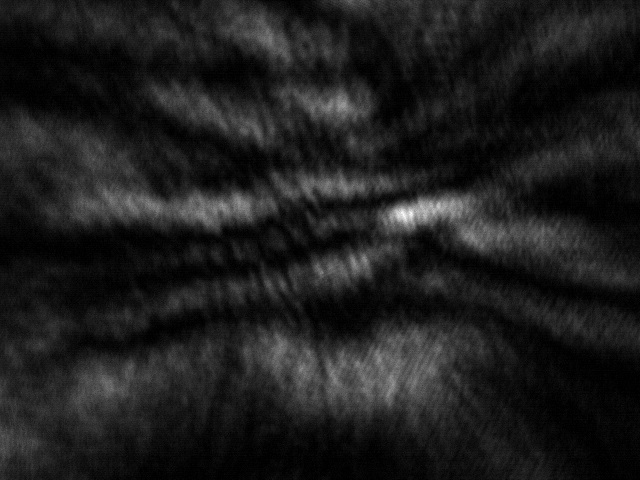
\includegraphics[width=\textwidth]{diffraction_image/2015040117594700158-2}
    \caption{s-polarizor}
  \end{subfigure}
  \caption{Diffraction images classified as Strip type}
\end{figure}
Through the pre-classification process, we have 957 image pairs in Cell folder, 1555 image pairs in Debris folder, and 488 pairs in Strip folder. To process these image data, we operate the JAVA application and set up the offset and angular direction parameters shown in Figure 2.9. 
\begin{figure}
\centering
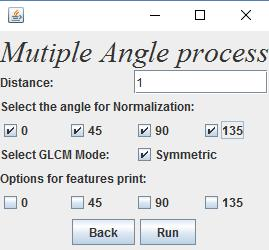
\includegraphics{java_panel}
\caption{JAVA application main panel}
\end{figure}
As it shown, the distance between two pixels is 1 and the application process the diffraction image data along with all directions. Because of having the symmetric checked, each value of an element in GLCM along each direction is doubled. In the meantime, the value of each element in GLCM is divided by the number of created GLCM, as well as normalized by the total amount of occurrences of valid reference pixel values. Eventually, the application generates three CSV files, Cell.CSV, Debris.csv, and Strip.csv, as the results that are used in the automated classification research later. 
\section{Conclusion}
In this section, we focus on the image texture analysis approach. As we discussed above, texture analysis is a common way to facilitate the analysis process. Within the texture analysis, GLCM is a popular and useful method to deal with the image texture analysis problems. It is proposed by Haralick\cite{Haralick} in 1973. The GLCM is created based on the spatial relations between two pixels of an image through counting the total number of occurrence of each pixel pair. The texture features are calculated from the GLCM to facilitate describing an image. In this research, we present the calculation of 20 texture features of images and apply 17 out of the total 20 features for automated classification experiment later. We implement JAVA application to verify MATLAB script and C++ tool but achieve three different versions of results. By applying black-box testing for all components of JAVA application, we confirmed the application has been implemented to meet all requirements. Through the operation of this application, all experiment image data are processed into texture features.  